\documentclass{article}

\usepackage{amsmath}
\usepackage{amssymb}
\usepackage{graphicx}
\usepackage{tikz}

\DeclareMathOperator{\erf}{erf}
\DeclareMathOperator{\Var}{Var}
\DeclareMathOperator{\Cov}{Cov}
\DeclareMathOperator{\E}{E}

\title{Clock steering in ntpd-rs}

\begin{document}

\maketitle

In NTP, each message sent to an NTP server gives a single response. For this round trip, the server reports back at what time it received the request and when it sent the response. These timestamps, together with when the client actually sent the request and response, give a measure of the offset between the clock of the client and the server, and of how long the network delay between them was.

Packet switching networks such as the internet or local Ethernet networks do introduce a lot of noise into these measurements though. Furthermore, a client may want to utilize the time from multiple servers so as to be able to deal with a server being either malicious or broken. To ensure network noise doesn't affect the local clock too badly, and to handle multiple servers, processing of the measurements is needed before the clock can be steered.

This paper describes the approach used in ntpd-rs to go from the raw measurements all the way to steering of the system clock. The main idea is to use a Kalman filter to filter the samples similar to what is proposed in \cite{giada2015}, combined with a selection approach and pop filter inspired by the filter specified in \cite{rfc5905}.

\section{Prerequisites and notation}

The rest of this paper assumes a comfort level with linear algebra to at least the level of calculating with matrices and vectors. We also assume some knowledge of probability theory.

In terms of notation, if $X$ is a random variable, we will denote its expectation value with $\E(X)$. We will denote the variance with $\Var(X) = \E((X-\E(X))^2)$, and if $Y$ is a second random variable, the covariance between $X$ and $Y$ will be denoted with $\Cov(X,Y) = \E((X-\E(X))(Y-\E(Y)))$.

We will also see random vectors. For an example, we call a 2-dimensional vector
\begin{align}
W &= \begin{pmatrix}
W_1\\
W_2
\end{pmatrix}
\end{align}
a random vector when its components $W_1$ and $W_2$ are random variables. For a random vector we define its covariance matrix as the matrix of the covariances between its components. For the example vector W, its covariance matrix is given by
\begin{align}
U &= \begin{pmatrix}
\Cov(W_1, W_1) & \Cov(W_1, W_2)\\
\Cov(W_2, W_1) & \Cov(W_2, W_2)
\end{pmatrix}\\
&= \begin{pmatrix}
\Var(W_1) & \Cov(W_1, W_2)\\
\Cov(W_1, W_2) & \Var(W_2)
\end{pmatrix}.
\end{align}

\section{Global architecture}

\begin{figure}[h]
\center{
	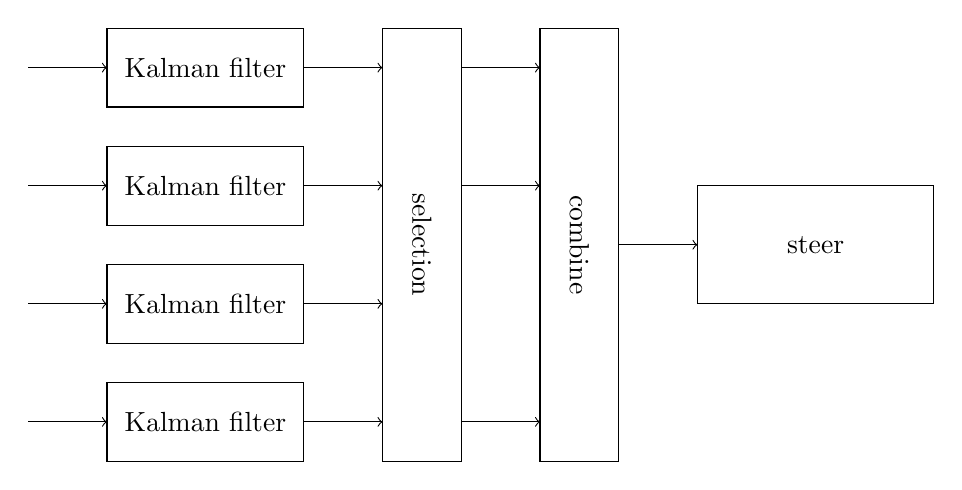
\begin{tikzpicture}
	\draw[->] (0, 0.5) -- (1, 0.5);
	\draw[->] (0, 2) -- (1, 2);
	\draw[->] (0, 3.5) -- (1, 3.5);
	\draw[->] (0, 5) -- (1, 5);
	\draw (1,0) rectangle (3.5, 1) node[pos = .5] {Kalman filter};
	\draw (1,1.5) rectangle (3.5, 2.5) node[pos = .5] {Kalman filter};
	\draw (1,3) rectangle (3.5, 4) node[pos = .5] {Kalman filter};
	\draw (1,4.5) rectangle (3.5, 5.5) node[pos = .5] {Kalman filter};
	\draw[->] (3.5, 0.5) -- (4.5, 0.5);
	\draw[->] (3.5, 2) -- (4.5, 2);
	\draw[->] (3.5, 3.5) -- (4.5, 3.5);
	\draw[->] (3.5, 5) -- (4.5, 5);
	\draw (4.5, 0) rectangle (5.5, 5.5) node[pos = .5, rotate=-90] {selection};
	\draw[->] (5.5, 0.5) -- (6.5, 0.5);
	\draw[->] (5.5, 3.5) -- (6.5, 3.5);
	\draw[->] (5.5, 5) -- (6.5, 5);
	\draw (6.5, 0) rectangle (7.5, 5.5) node[pos = .5, rotate=-90] {combine};
	\draw[->] (7.5, 2.75) -- (8.5, 2.75);
	\draw (8.5, 2) rectangle (11.5, 3.5) node[pos = .5] {steer};
	\end{tikzpicture}
}
\caption{Diagram with the parts of the ntpd-rs clock control filter. The arrows on the left represent the measurements from the (in this case) 4 time sources coming in.}
\end{figure}

The clock control filter of ntpd-rs consists of 4 stages.

First, on a per time source basis, a Kalman filter is used to estimate the offset and frequency error as compared to that specific time source.
During this stage, the remote clock is treated as ground truth and any uncertainty with respect to UTC it reports is ignored.
Sections~\ref{sec:Kalmanfilter}-\ref{sec:additionalchecks} describe this Kalman filter.

Next, we compare all time sources and see which subset of them is in agreement.
We also check for each time source whether it is of sufficient quality to use.
Selection criteria, as well as the used algorithm, are detailed in Section~\ref{sec:selection}.

Having selected which sources to use, these sources' measurements are averaged to produce an estimate of the clock offset.
The procedure for the averaging is described in Section~\ref{sec:averaging}.

Finally this clock offset, and the error bounds on it, are used to steer the system clock to bring it in closer agreement with the remote time sources.
We steer primarily using frequency adjustment, the exact procedure used is described in Section \ref{sec:steering}.

\section{Kalman filter}\label{sec:Kalmanfilter}

To estimate offset and frequency error with regard to a remote clock, we use a Kalman filter to interpret the measurements.
Although we regard the remote clock as ground truth for this filter, we choose to parameterize the state as a function of local time $t_l$.
We will use $t_r$ to denote the time indicated by the remote clock.
The remote time corresponding to local time $t_l$ is denoted as $t_r(t_l)$.
For convenience we will use the same symbols as Wikipedia for the equations for a Kalman filter given below.

Our state model consists of two parameters: The offset $\Delta$ and the frequency error $\omega$ with respect to the remote clock. These are defined such that
\begin{align}
\Delta(t_l) &= t_r(t_l) - t_l, \\
\omega(t_l) &= \lim_{t_l' \rightarrow t_l}\frac{t_r(t_l') - t_r(t_l)}{t_l' - t_l} - 1 = \frac{\mathrm{d} t_r}{\mathrm{d} t_l}(t_l) - 1.
\end{align}
Combined, these form our state vector
\begin{align}
x(t_l) &= \begin{pmatrix}
\Delta(t_l)\\
\omega(t_l)
\end{pmatrix}.
\end{align}
We will use the symbol $P$ to refer to the covariance matrix for this state.

Given these definitions, the update matrix for when a local timespan $\delta$ has passed is given by
\begin{align}
F(\delta) &= \begin{pmatrix}
1 & \delta\\
0 & 1
\end{pmatrix}.
\end{align}
Updating the Kalman filter's state from $t_l$ to $t_l+\delta$ is then given by
\begin{align}
x(t_l+\delta) &= F(\delta)x(t_l),\\
P(t_l+\delta) &= F(\delta)P(t_l)F(\delta)^\mathrm{T} + Q(\delta).
\end{align}
Here we will keep the process noise matrix $Q(\delta)$ general, stating only that we require two update steps of sizes $\delta_1$ and $\delta_2$
to give the same result as a single update step of size $\delta_1 + \delta_2$ when no measurement is done in between.
A detailed treatment of our noise model is given in Section~\ref{sec:processnoise}.

Measurements from the NTP protocol give us an immediate estimate of $\Delta$. Letting $z$ be the (1-element) vector with this measurement,
and $R$ its covariance matrix (which in this case is simply an estimate of the variance of the measurement).
This corresponds to a measurement matrix of the form
\begin{align}
H &= \begin{pmatrix}
1 & 0
\end{pmatrix}.
\end{align}
Such a measurement can be incorporated into the filter by first calculating
\begin{align}
y &= z - Hx,\\
S &= H P H^\mathrm{T} + R,\\
K &= P H^\mathrm{T} S^{-1},
\end{align}
which allows us to update the state through
\begin{align}
x' &= x + Ky,\\
P' &= (I - K H)P,
\end{align}
where $x'$ and $P'$ denote the post-measurement state and covariance matrix, and $I$ is the identity matrix.

The intermediate matrices $S$ and $K$ do have intuitive interpretations. $S$ gives an estimate for how $y$ is expected to be distributed, giving the covariance matrix of the vector $y$, which is expected to have a mean of $0$. The matrix $K$, also known as the Kalman gain, gives a measure for how much each part of the state should be affected by each part of the difference between measurement and prediction.

We will use the symbols given here for the various matrices involved in the Kalman filter throughout the rest of this paper.

\section{Process noise}\label{sec:processnoise}

For our Kalman filter we need estimates for the process noise $Q$ and measurement noise $R$. Let us start by first considering the process noise.

Working out the requirement that a single large step should give the same as two smaller steps, we find that for all $x$, (symmetric) $P$, $\delta_1$ and $\delta_2$
we should have
\begin{align}
F(\delta_1 + \delta_2)x = F(\delta_2)F(\delta_1)x,\\
F(\delta_1 + \delta_2)PF(\delta_1 + \delta_2)^\mathrm{T} + Q(\delta_1+\delta_2) =\nonumber\\
F(\delta_2)(F(\delta_1)PF(\delta_1)^\mathrm{T} + Q(\delta_1))F(\delta_2)^\mathrm{T} + Q(\delta_2).
\end{align}

The first follows trivially from the identity
\begin{align}
F(\delta_1 + \delta_2) = F(\delta_2)F(\delta_1).
\end{align}

This same identity can also be used to simplify the second requirement to
\begin{align}
Q(\delta_1+\delta_2) = F(\delta_2)Q(\delta_1)F(\delta_2)^\mathrm{T}+Q(\delta_2).
\end{align}
Writing out this equation in the components $q_{ij}(\delta_t)$ (using that $Q$ is symmetric) gives
\begin{align}
q_{11}(\delta_1+\delta_2) &= q_{11}(\delta_1) + q_{11}(\delta_2) + 2\delta_2q_{12}(\delta_1)+\delta_2^2q_{22}(\delta_1),\\
q_{12}(\delta_1+\delta_2) &= q_{12}(\delta_1) + q_{12}(\delta_2) + \delta_2q_{22}(\delta_1),\\
q_{22}(\delta_1+\delta_2) &= q_{22}(\delta_1) + q_{22}(\delta_2).
\end{align}
Solving these equations, we find that there need to be constants $A$, $B$ and $C$ such that 
\begin{align}
q_{11}(\delta) &= \frac{A}{3}\delta^3 + B\delta^2 + C\delta,\\
q_{12}(\delta) &= \frac{A}{2}\delta^2 + B\delta,\\
q_{22}(\delta) &= A\delta.
\end{align}

The $A$ contribution to $Q$ corresponds with a random walk noise of the frequency with infinitesimal steps.
Similarly, the $C$ contribution is a random walk noise of the phase, without any underlying frequency change.
\footnote{For an explanation of the names of these noise components, see Appendix~\ref{sec:randomwalk}.}

The $B$ contribution to the noise is somewhat harder to interpret. It corresponds to a form of correlation between the infinitesimal steps
of the frequency and phase random walk noise. As such, its maximum amplitude is actually limited by $|B| < \sqrt{AC}$.
Furthermore, it has no effect on the expectations for Allan deviation and modified Allan deviation.
This makes it tricky to see whether it even corresponds to an actual noise component in the real world.

For our implementation, we assume process noise is purely made up from the $A$ component. Doing this will enable our implementation to dynamically
estimate its own process noise.

Our assumption is reasonable for NTP as for modern computer oscillators, the phase random walk noise is dwarfed by channel noise until frequency random
walk becomes dominant. 
We assume the $B$ component to be irrelevant based on the observations in the previous section.

\subsection{Estimating process noise}

The process noise for our Kalman filter will depend both on characteristics of the remote clock as well as those of the local oscillator.
As such, although we can estimate a reasonable value as a starting point, it is unlikely that all computers will perform at their best with
a single estimate for the frequency random walk noise.

To solve this, we dynamically determine the process noise at runtime.
The filter is started with an initial estimate of the wander noise, by default $A=10^{-16}$.
Then, as each measurement comes in, we calculate the probability $p$ of getting a measurement that close, or closer, to our state estimate.
Based on the distribution of $p$ we can then determine whether our estimate of the noise is low (if $p$ consistently is large) or high (if $p$ consistently is small) and adjust $A$ accordingly.

Concretely, we keep a counter $M$ with a starting value of $0$. If $p$ is smaller than $\frac{1}{3}$, we subtract one from $M$.
Conversely, if $p$ is larger than $\frac{2}{3}$, we add one to $M$. Finally, if $p$ is between $\frac{1}{3}$ and $\frac{2}{3}$, we move $M$ one towards $0$.

If $M$ gets above $16$, we reset $C$ to $0$ and multiply $A$ by four (doubling the standard deviation of the noise).
Similarly, if $M$ gets below $-16$, we divide $A$ by four.
Waiting for multiple measurements before adjusting our uncertainty estimates ensures that our estimate doesn't keep changing.
This is further helped by having the region between $\frac{1}{3}$ and $\frac{2}{3}$ push $M$ towards $0$, as this works to keep $|M|$ small.

Of course, $p$ shows problems with the process noise only when it is a significant fraction of the total measurement noise.
As such, if the measurement noise is more than $\frac{9}{10}$ the total noise of the difference between measurement and prediction, a $p$ smaller
than $\frac{1}{3}$ no longer lowers $M$, instead also pushing it towards $|M|$, to avoid becoming overly optimistic on process noise if the
measurement noise estimate is somewhat pessimistic.

\subsubsection{Calculation details for $p$}

To find $p$, first note that $S$ is effectively the covariance matrix of the difference $y$ between the prediction from the filter for the measurement and
the actual measured value. This implies that $y S y^\mathrm{T}$ is distributed according to a chi-squared distribution with one degree of freedom.

The cumulative density function for the chi-squared distribution with one degree of freedom is given by $1-\erf\left(\sqrt{\frac{x}{2}}\right)$,
where $\erf(x)$ denotes the error function.
Combining this with the above, we find
\begin{align}
p = 1 - \erf\left(\sqrt{\frac{y S y^\mathrm{T}}{2}}\right).
\end{align}

\section{Measurement Noise}\label{sec:measnoise}

To complete the parameters for our filter, we also need an estimate of the measurement noise.
We will construct this using the variance in the delay in the NTP measurements.

\begin{figure}[h]
\center{\includegraphics[width=0.8\textwidth]{measurement.png}}
\caption{Schematic diagram of an NTP measurement.}\label{fig:measurement}
\end{figure}

To start, each NTP measurement consists of $4$ timestamps, $t_1$ through $t_4$.
These give two time differences, the forward offset $r_1 = t_2 - t_1$ and the backward offset $r_2 = t_4 - t_3$.
The primary assumption behind NTP is that when the client and server clocks are synchronized, $r_1 = r_2$.

Hence, these two time differences give rise to two estimates: the offset $\Delta = \frac{r_1 - r_2}{2}$ and the delay $d = r_1 + r_2$.
We now make two crucial assumptions: 
First, the forward and backward offsets are independent random variables (i.e. $\Cov(r_1, r_2) = 0$)
And second, the mean value of the delay $d$ is constant over multiple measurements.

The first assumption allows us to relate the variance of the offset to that of the delay:
\begin{align}
\Var\left(\frac{r_1-r_2}{2}\right) = \frac{1}{4}\left(\Var(r_1) + \Var(r_2)\right) = \frac{1}{4}\Var(r_1+r_2).
\end{align}

Then, the third assumption permits us to estimate the variation of the delay from the sample variance over multiple measurements.
We implement this in ntpd-rs by keeping a ring buffer with the last 8 values for the delay.
A quarter of the sample variance of these 8 measurements is then used as the estimate for the variance in the matrix $R$ when incorporating a measurement.

\section{Additional filtering and checks}\label{sec:additionalchecks}

In the previous section we described the main Kalman filter used to estimate clock differences from the measurements.
There are a few additional minor checks done in the Kalman filter stage as well.

First, at each measurement the filter checks the relationship between the local wall time clock and the local monotonic clock.
It can estimate what their difference should be based on how the clock has been steered by ntpd-rs.
As such, any unexpected differences are indications that some other process has modified the local clock.
Upon detecting such differences, the filter is reset to a startup state to ensure more rapid recovery from unexpected clock changes.

Second, before each measurement is fully processed, the delay is checked against the buffer of previous delays.
If it is far larger than expected (five standard deviations above the mean with the default configuration) it is ignored.
Only if a second sample in a row has a delay much larger than expected then this second sample is actually processed.
This simple pop filter allows ignoring of one-time upsets in the network which would otherwise degrade precision estimates for quite a long time.

\section{Selection}\label{sec:selection}

The Kalman filter stage gives us for each time source an offset and frequency error.
We now need to make a choice which of these sources to actually use to synchronize the clock.

For this, we first construct for each source a range in which we estimate its actual offset to be.
This by default consists of twice the output uncertainty of the Kalman filter, plus a quarter of the mean delay to that time source.
If this range is larger than the maximum allowed source uncertainty (0.25 by default), we will disregard this source for now.

Next we search for the largest set of agreeing sources. We consider two sources to be in agreement when their likely ranges of offsets overlap,
and consider a set of sources to be in agreement if all possible pairs in the set are in agreement.

This set is located by first creating a list of all the endpoints of the likely offset ranges of all the sources.
Next, this list of endpoints is sorted in order of offset.
By going over the list in this order with a sweepline algorithm we can find an offset within the intersection of the ranges of a maximum set of sources.
Once we have one such offset, we then go over the list of sources a second time, selecting all sources whose range contains that offset for synchronization.

If a majority of all sources passing the range size criteria, and be of sufficient size (by default 3), then this set is flagged as actually usable for
steering the clock.
If there is no majority agreeing on the current time, or if that majority is too small, the next stages (averaging and steering) are not executed.
In such cases, the clock is not steered until a sufficient number of time sources again agree on the current time.

\section{Averaging}\label{sec:averaging}

Having a group of time sources that can agree on an offset for the clock, we next need to calculate which offset (and frequency error) they actually agree on.
For this, we use the error estimates produced by the Kalman filter, to which we add the time sources own estimate of its error.
This gives for each time source $i$ a vector $x_i = \begin{pmatrix}\Delta_i\\\omega_i\end{pmatrix}$ with its estimate of the offset and frequency error,
and a covariance matrix $P_i$ giving the uncertainty of that estimate.

The formulas for combining the estimates and uncertainties of two time sources are similar to those for incorporating a measurement in the Kalman filter:
\begin{align}
\bar{x} &= x_i + P_i(P_i+P_j)^{-1}(x_j - x_i),\\
\bar{P} &= P_i(P_i+P_j)^{-1}(x_j - x_i).
\end{align}
To combine all the measurements, these formulas are repeatedly applied to incorporate each measurement into a running average.

\section{Clock steering}\label{sec:steering}

Having combined all selected measurements, the result can now be used to steer the clock.
For this, we extract the offset and frequency error, and their respective uncertainties.
The correlation in the uncertainty between offset and frequency error is currently not used.

There are then three possible scenarios. First, if there is a very large offset observed (greater than 10 milliseconds), 
it will be corrected with a step in the local clock.
Step corrections are limited by both the step limit and the accumulated step limit, which limit the maximum one-time step change in the clock as well
as the accumulated steps over time. If either of these limits is exceeded, the software will exit with an error to alert the system administrator
that there may be a potential security problem.

If the offset is not so large, but still larger than twice the uncertainty in the offset, we correct the offset by running the clock a bit slower or a bit
faster for at least 8 seconds, or for however long is needed to correct the offset with a maximum frequency deviation of 200ppm. However, to deal with
the fact that the threshold actually makes it somewhat more likely that we are looking at an extreme value of the distribution, we don't correct the entire
offset, but by default leave an offset of the same size as the uncertainty after the change, in the same direction as the original offset.

During both of the above offset steering steps, the entire frequency error is corrected for. This is done either separately when doing a step, or as part
of the frequency changes for the continuous clock change. However, if neither is needed after doing a measurement, a separate correction for the frequency
is done. With the standard settings, this corrects away the entire observed frequency error.

In ntpd-rs, all the numbers named above can be configured to have different values, and for frequency a similar threshold-leftover scheme can be used as for offset.
The defaults for the latter are just both set to 0.

\section{Poll interval selection}

There is one final thing we haven't touched on yet, and that is how ntpd-rs chooses how often to ask each server for the time. This is done in two stages. First, the algorithm selects a desired poll interval for all time sources. Then, on a per time source basis, this is adapted to deal with server-indicated limits on how often we may ask, and backoffs that kick in on failures. Here, we will focus only on the selection of a desired poll interval.

For this, first a desired poll interval is selected for each time source such that the measurement noise is between 40 and 60 percent of the total uncertainty on the difference between prediction and measurement. This is again done with a counter mechanism similar to the process noise estimation. This time, any measurement for which less than 40 percent of the difference uncertainty is measurement is a vote for a longer poll interval, anything where it is more than 60 percent is a vote for a shorter poll interval and anything in between pushes the counter back to 0.

Then the overall desired poll interval is the minimum of the desired poll intervals of all the time sources. This is currently done as a global indicator primarily because of limitations in the architecture of ntpd-rs. In the future, this may change to a desired poll interval that is different for each source.

Note also that, as in the case of process noise estimation, the specific numbers mentioned above are configurable. The values above are the current default values used by ntpd-rs.

\section{Performance}

We evaluated the performance of the new algorithm against the default settings of chrony version 4.0, another NTP client. For this, we connected a Raspberry Pi 4 via a switch to a local GPS-connected NTP server (an Endrun Ninja). Both the Raspberry Pi and the NTP server were configured to produce pulse per second outputs.

For each test, the NTP client under test was started on the Raspberry Pi with a fixed poll interval of 1 second and allowed to stabilize over a period of at least half an hour. Then, the offset between the pulse per second signals of the Raspberry Pi were measured for one hour. The results of these measurements are shown in Figure~\ref{fig:offset-time}. Both chrony and ntpd-rs were configured to use the local server as only time source, but otherwise used their default configuration.

\begin{figure}[h]
\includegraphics[width=0.5\textwidth]{offset-ntpd-rs.png}\includegraphics[width=0.5\textwidth]{offset-chrony.png}
\caption{Offset of the Raspberry Pi running ntpd-rs (left) and chrony (right) over a time period of 1 hour, compared to the server they were synchronizing to.}\label{fig:offset-time}
\end{figure}

We haven't corrected in any way for asymmetries in the setup on the network layer, so any difference between the average offset to the server and the Raspberry Pi cannot be interpreted as significant advantages for either ntpd-rs or chrony. However, the deviation from this mean does provide a clear indication of synchronization quality. For chrony, the deviation is $3.6$ microseconds. For ntpd-rs it is $1.8$ microseconds. From this we conclude that ntpd-rs is at least on par with chrony, and likely slightly better.

\bibliographystyle{plain}
\bibliography{algorithm}

\appendix
\section{Random walk noise}\label{sec:randomwalk}

In the analysis of the process noise we identified two of the three components of the process noise as phase and frequency random walk noise respectively. In this appendix, we discuss where this term comes from, and the intuitive model behind it.

Consider the following process: We start at 0 and at each timestep $i$ we make a random step $X_i$. We assume that the steps are independent ($\Cov(X_i, X_j) = 0$ if $i \ne j$) and all have the same variance $\Var(X_i) = s$. If each timestep has length $D$, then after a timespan $T = ND$ the result $X(T) = \sum_{i=1}^N X_i$ has a variance $\Var(X) = Ns = \frac{T}{D} s$.

If we now make the timesteps smaller, but keep $b = \frac{s}{D}$ constant the variance of $X(T)$ also stays constant. In the limit where the timesteps length goes to $0$, we still get the same form for the variance of $X$ over time: $\Var(X(T)) = bT$, which is the form we see coming back in the variance of the phase and frequency respectively in Section~\ref{sec:processnoise}.

There is one further detail to further discuss, which is the contribution of frequency noise to the phase noise. Because the phase is effectively the integral of the frequency, any frequency noise also shows up as variance in the phase. Going back to a model with steps of a finite duration the variance of the phase as a consequence of frequency noise can be calculated similar to above. We leave the actual calculation as an exercise for the reader.

\end{document}
